\documentclass[12pt]{article}

\usepackage[top=1in, bottom=1in, left=1.2in, right=1in]{geometry}
\pagestyle{plain}
\linespread{1.5}

\usepackage[T1]{fontenc}
\usepackage[utf8]{inputenc}
\usepackage[english]{babel}
\usepackage{mathptmx}
\usepackage{graphicx}
\usepackage{floatflt}
\usepackage{blindtext}
\usepackage{enumitem}
\usepackage{subfig}
\usepackage{listings}
\usepackage{listingsutf8}
\usepackage{parskip}
\usepackage{amsmath}
\usepackage{framed}
\usepackage{minibox}
\usepackage{float}
\usepackage{wrapfig}
\usepackage{longtable}
\usepackage[strict]{changepage}
\usepackage{pgfplots}
\usepackage{hyperref}
\usepackage{tikz}
\usepackage{listings}
\usetikzlibrary{matrix}
\pgfplotsset{width=11cm,compat=1.9}
\usepgfplotslibrary{external}
\tikzexternalize

\hypersetup{
    colorlinks=true,
    linkcolor=blue,
    filecolor=magenta,      
    urlcolor=cyan,
}

\usepackage{subfiles}

\begin{document}
\title{title}
\author{author}
\date{date}

\begin{titlepage}
\begin{figure}[t]
    \centering
\includegraphics[width=0.3\textwidth]{./images/COMSATS.jpg}
\end{figure}
\begin{center}
    \textsc{ \LARGE{Comsats University, Islamabad \\}}
	\textsc{ \LARGE{Data Communication and Networks\\ }}
	\textnormal{ \LARGE{Lab Project Report\\}}
	\vspace{20mm}
	\fontsize{10mm}{7mm}\selectfont 
	\textup{FullStack FTP Server with Socket-based Intercommunication}\\
	\textsc{ \LARGE{Class: 5-B\\ }}
\end{center}

\vspace{15mm}

\begin{minipage}[t]{0.47\textwidth}
	\textnormal{\large{\bf Members:\\}}
	{\large Syed Muhammad Irtesam\\ Mutahhar Bin Muzaffar\\ Uzayr Qamar}
\end{minipage}\hfill\begin{minipage}[t]{0.47\textwidth}\raggedleft
	\textnormal{\large{\bf Reg. No:\\}}
	{\large FA17-BCS-088\\ FA17-BCS-058\\ FA17-BCS-096}
\end{minipage}

\vspace{10mm}

\centering{\large{Project Supervisor: Ahmed Kakakhail}}

\end{titlepage}

\tableofcontents

\pagebreak

\setlength{\parindent}{0pt}
\setlength{\parskip}{1em}

\section{Introduction}
This project intends to provide FTP-based authentication on a file server
while allowing users to remotely download and upload files to the server.
We will utilize sockets to simulate a connection between two FTP clients by providing a
simple terminal interface for file transfer between FTPs. On the other hand, we will provide
users of the FTP a fully functional GUI to download and upload files to a central FTP server 
without the need of a command-line interface.
This solves a scenario where a company might utilize multiple FTP servers in their
infrastructure. Thus, we are covering all paradigms of FTP usage in tech sectors.
By building a neat and streamlined web interface for this project,
we can do away with clunky and limited tools like FileZilla and SyncTrayzor.

\section{Functional Requirements}
This system solves the following functional requirements:
\begin{itemize}
	\item Provide application-scaling user authentication
	\item Provide a streamlined interface for management of files
	\item Provide easy controls for file upload and download
	\item Display basic info about all files in tabulated form
	\item Provide dynamic and accurate front-end updates about file-system to the user
	\item Allow multiple FTP servers to inter-communicate
	\item Allow remote clients to access files through command-line
	\item Provide a simple RESTful API that can be easily exposed with proper OAuth
\end{itemize}

\section{Tools and Technologies}
\subsection{Tools}
\begin{itemize}
	\item Visual Studio Code
	\item Ubuntu
	\item Windows Powershell
	\item apt/pacman/chocolatey
	\item cURL (HTTP Client)
	\item Windows Subsystem for Linux (WSL)
	\item IDEA IntelliJ
	\item Git Bash (Github)
	\item LaTeX/TeX Live
\end{itemize}
\subsection{Technologies}
\begin{itemize}
	\item NodeJS
	\item ExpressJS
	\item VueJS
	\item OpenJDK
	\item Vuex/Vue Router
	\item bulma.io
	\item yarn
	\item ESLint
	\item webpack
	\item babel.js
	\item CSS Loader/SASS Loader/Vue Loader
\end{itemize}

%\pagebreak

\section{Screenshots}
\subsection{FTP Login Page}

\includegraphics[scale=0.3]{images/login.png}
\subsection{FTP Main Interface}
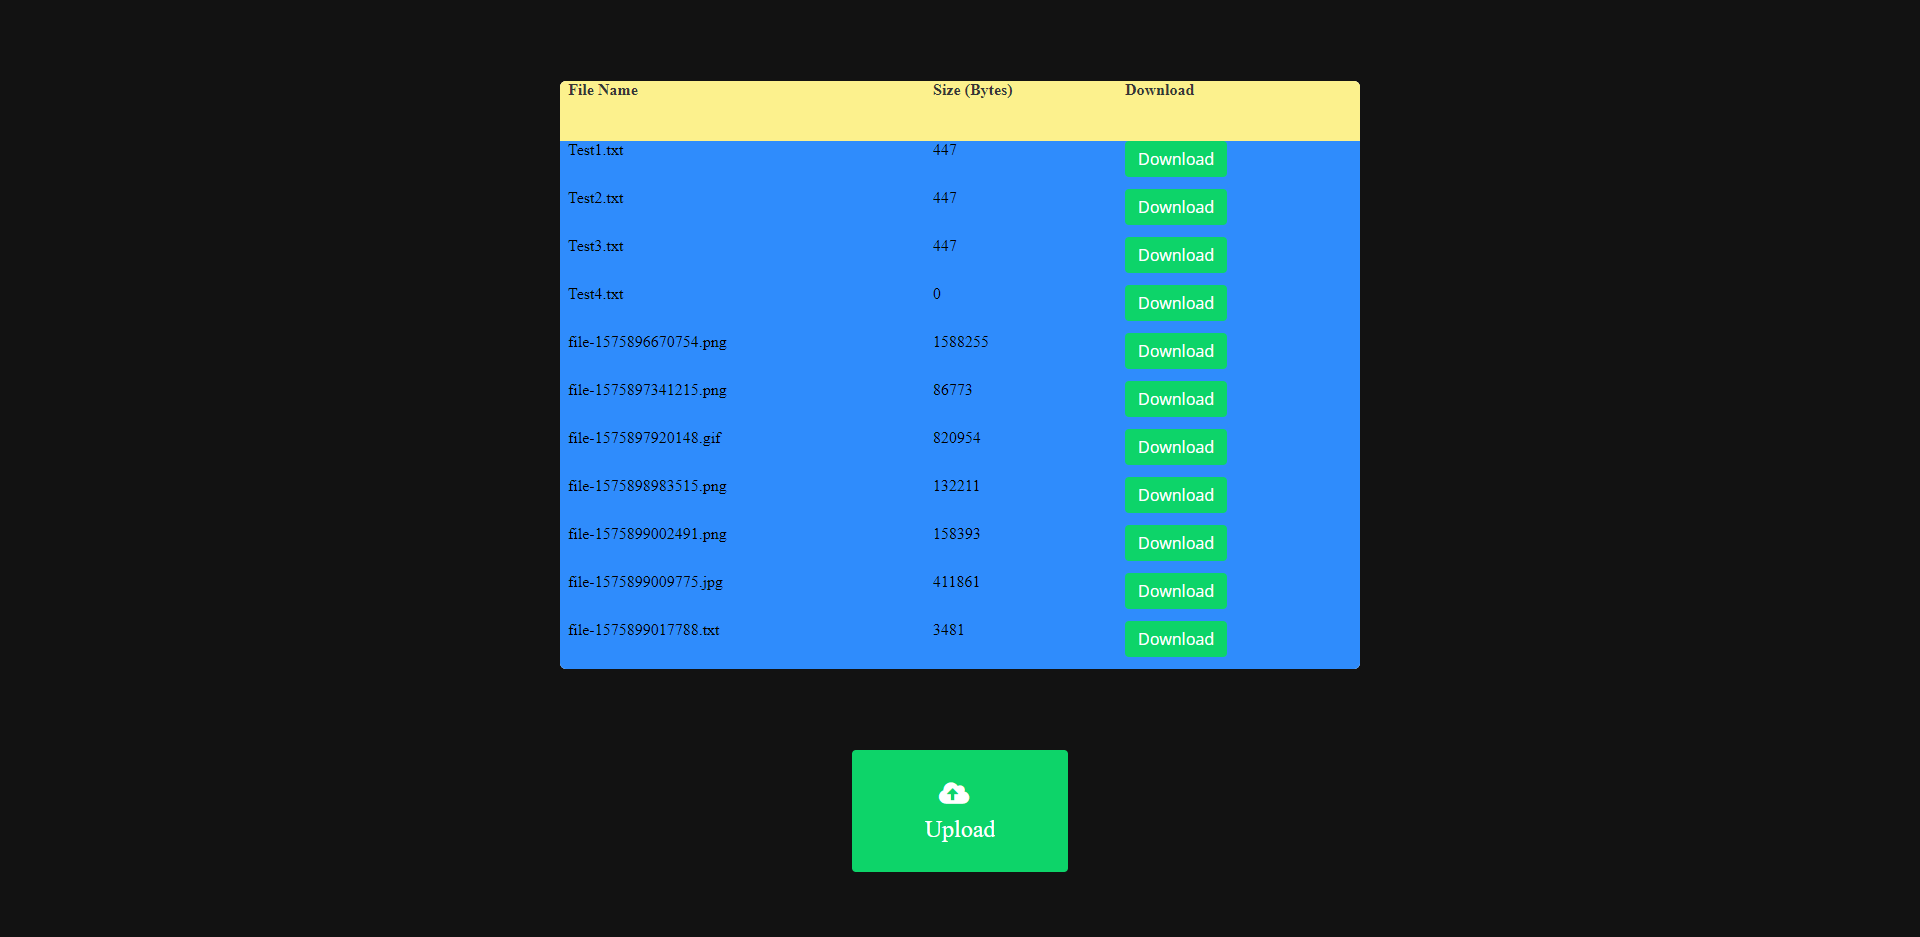
\includegraphics[scale=0.3]{images/dirlist.png}
\subsection{Terminal with FTP loaded}
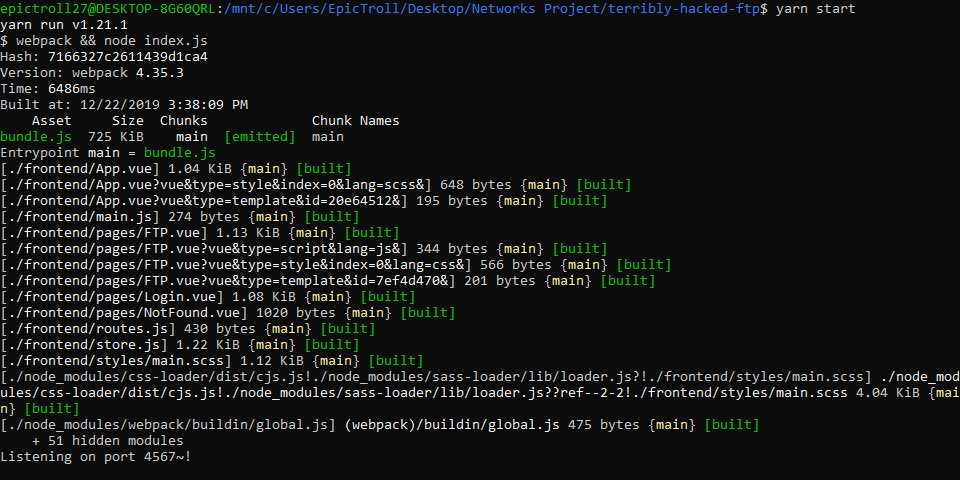
\includegraphics[scale=0.6]{images/bash.png}
\subsection{Java FTP Server Socket}
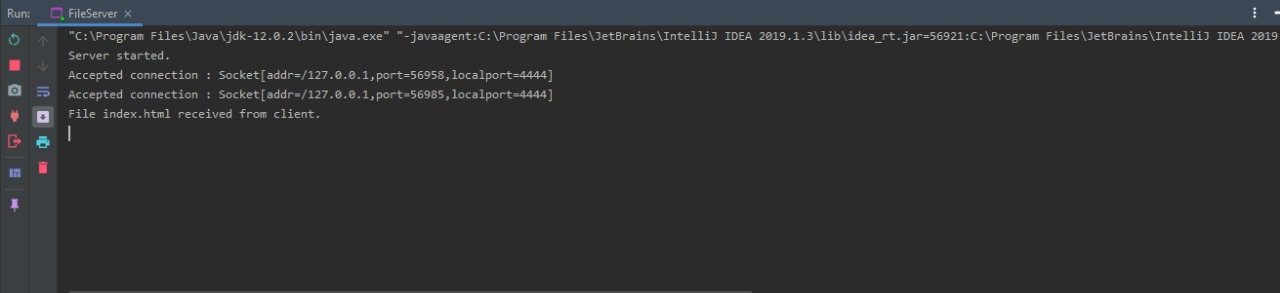
\includegraphics[scale=0.4]{images/server.jpeg}
\subsection{Java FTP Client Socket}
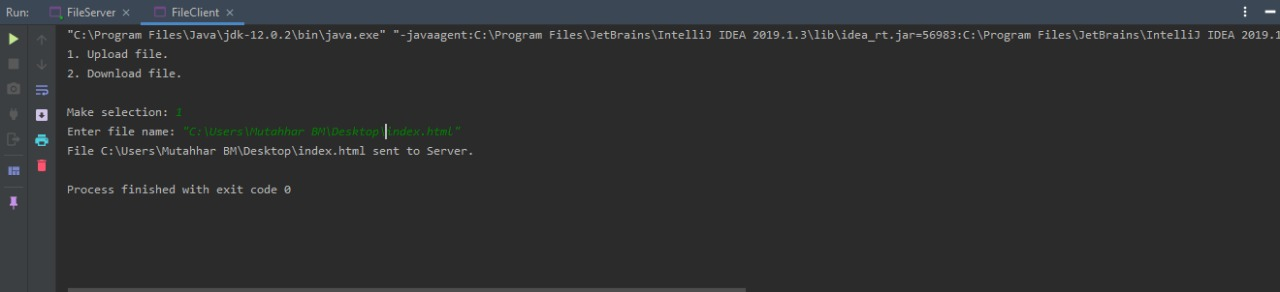
\includegraphics[scale=0.4]{images/client.jpeg}

\section{Getting Started}
After installing NodeJS, yarn, IDEA IntelliJ, follow these instructions from the README.md file included in the project:
\begin{verbatim}
	#Copy and edit config
	$ cp sample.config.js config.js && $EDITOR config.js
	# Install dependencies
	$ yarn
	# Build and run
	$ yarn start
\end{verbatim}

After the application is deployed, you should start the Java server and open a client connection to receive files 
from other FTPs. The ports and IP addresses must be edited manually inside the Java files.

\section{Source Code}

\subsection{index.js}
\begin{verbatim}
	const fs = require('fs');
	const path = require('path');
	const express = require('express'); // Web server
	const config = require('./config'); // Generic configuration
	const sirv = require('sirv'); // Static file middleware
	const api = require('./routes/api');
	
	const indexPage = fs.readFileSync(path.join(config.publicDir, 'index.html'));
	
	// Define the main application
	const app = express({
		onNoMatch: (request, response) => response.end(indexPage),
	});
	
	// Set up global middlewares
	app.use(sirv(config.publicDir, {dev: true}));
	
	// Register the API routes and auth routes
	app.use('/api', api);
	app.set('view engine', 'ejs');
	
	// Start the server
	app.listen(config.port, () => {
		console.log(`Listening on port ${config.port}~!`);
	});
\end{verbatim}

\subsection{api.js}
\begin{verbatim}
	const apiApp = require('express')();
	const fs = require('fs');
	const config = require('../config');
	const path = require('path');
	const util = require('util');
	const multer = require('multer');
	
	const storage = multer.diskStorage({
		destination: config.serverDir,
		filename: function(req, file, cb){
		  cb(null,file.fieldname + '-' + Date.now() + path.extname(file.originalname));
		}
	  });
	
	  const upload = multer({
		storage: storage,
	  }).single('file');
	
	apiApp.get('/dirlist', (req, res) => {
		let dirArr = [];
		let files = [];
		const readDir = util.promisify(fs.readdir);
		const stat = util.promisify(fs.stat);
	
		readDir(config.serverDir).then(async (items)=> {
			files = items.slice(items);
		}).then(async () => {
			var count = 0;
			for (var i=0; i<files.length; i++) {
				var file = config.serverDir + '/' + files[i];
				const promise = await stat(file).then((data)=> {
					return {
						"id" : ++count,
						"name": path.basename(file),
						"size": data["size"].toString(),
					};
				});
				dirArr.push(promise);
			}
		}).then(()=> {
			res.json(dirArr);
			res.end();
		});
	});
	
	apiApp.get('/download/:fileName', (req,res) => {
		const file = config.serverDir + '/' + req.params.fileName;
		res.download(file);
	});
	
	apiApp.post('/upload', (req,res) => {
		upload(req, res, (err) => {
			if (err) {
				throw err;
			}
			res.end();
		  });
	});
	
	
	
	function checkFileType(file, cb){
		// Allowed ext
		const filetypes = /jpeg|jpg|png|gif/;
		// Check ext
		const extname = filetypes.test(path.extname(file.originalname).toLowerCase());
		// Check mime
		const mimetype = filetypes.test(file.mimetype);
	  
		if(mimetype && extname){
		  return cb(null,true);
		} else {
		  cb('Error: Images Only!');
		}
	  }
	
	module.exports = apiApp;
\end{verbatim}

\subsection{Vuex Store}
\begin{verbatim}
	import Vue from 'vue';
	import Vuex from 'vuex';
	const axios = require('axios');
	
	Vue.use(Vuex);
	
	async function makeRequest (path, method = 'GET', body) {
		if (typeof body === 'object' && body != null) {
			body = JSON.stringify(body);
		}
		try {
			const result = await fetch(path, {method, body});
			if (!result.ok) {
				const json = await result.json();
				throw json.error;
			}
			if (result.status === 204) {
				return;
			}
			return await result.json();
		} catch (error) {
			window.alert(error);
			throw error;
		}
	}
	
	const store = new Vuex.Store({
		state: {
			fileData: null,
			auth: false,
			downloadedFile: null,
		},
		mutations: {
			GET_FILES (state,fileData) {
				state.fileData = fileData;
			},
		},
		getters: {
			isAuth(state) {
				return state.auth;
			},
		},
		actions: {
			async getFiles({commit}) {
				const files = await makeRequest('/api/dirlist');
				commit('GET_FILES',files);
			},
			async downloadFile({commit},fileName) {
				setTimeout(() => {
					const response = {
					  file: `/api/download/${fileName}`,
					};
					window.open(response.file);
				  }, 50);
			},
		},
	});
	
	export default store;
\end{verbatim}

\section{Login.vue}
\begin{verbatim}
	<template>
	<section class="hero is-primary is-fullheight">
	  <div class="hero-body">
		<div class="container">
		  <div class="columns is-centered">
			<div class="column is-5-tablet is-4-desktop is-3-widescreen">
				<div class="field">
				  <label for="" class="label">Username</label>
				  <div class="control has-icons-left">
					<input type="text" placeholder="FTP Username"
					 v-model="username" class="input" required>
					<span class="icon is-small is-left">
					  <i class="fa fa-envelope"></i>
					</span>
				  </div>
				</div>
				<div class="field">
				  <label for="" class="label">Password</label>
				  <div class="control has-icons-left">
					<input type="password" placeholder="*******"
					 v-model="password" class="input" required>
					<span class="icon is-small is-left">
					  <i class="fa fa-lock"></i>
					</span>
				  </div>
				</div>
				<div class="field">
				  <button @click="doAuth" class="button is-success">
					Login
				  </button>
				</div>
				<div class="field">
				  <i class="label">{{message}}</i>
				</div>
			</div>
		  </div>
		</div>
	  </div>
	</section>
	</template>
	
	<script>
	const config = require('../../config');
	
	export default {
	  data () {
		return {
		  username: '',
		  password: '',
		  message: '',
		}
	  },
	  methods: {
		doAuth() {
		  const user = config.users.admin;
		  if (user.username==this.username && user.password == this.password) {
			this.$router.push({path:'/FTP'});
		  }
		  else {
			this.message = "Wrong username or password.";
		  }
		},
	  },
	}
	</script>
\end{verbatim}

\subsection{FTP.vue}
\begin{verbatim}
	<template>
	<section class="hero has-background-black-bis is-fullheight">
	  <div class="hero-body">
		<div v-if="fileData" class="container">
		<table class="is-full-width is-scrollable">
		  <thead>
			<tr>
			  <th>File Name</th>
			  <th>Size (Bytes)</th>
			  <th>Download</th>
			</tr>
		  </thead>
		  <tbody v-for="files in fileData" :key="files.id"
		   class="has-background-primary">
			<tr>
			  <td>{{files.name}}</td>
			  <td>{{files.size}}</td>
			  <td><button v-on:click="downloadFileSubmit(files.id)"
			   class="button is-success">Download</button></td>
			</tr>
		  </tbody>
		</table>
	  </div>
	  </div>
	  <div class="container">
	  <div class="file is-boxed is-centered is-large is-success">
		  <label class="file-label">
		  <input v-on:change="uploadFile" class="file-input" type="file"
		   name="file" id="file">
		  <span class="file-cta">
			<span class="file-icon">
			  <i class="fas fa-cloud-upload-alt"></i>
			</span>
			<span class="file-label">
			  Upload
			</span>
		  </span>
		  </label>
		</div>
		</div>
	</section>
	</template>
	
	<script>
	import {mapState, mapGetters, mapActions} from 'vuex';
	const axios = require('axios');
	
	export default {
	  data () {
		return {
		  file: '',
		}
	  },
	  computed: {
		...mapState(['fileData','auth']),
		...mapGetters(['isAuth']),
	  },
	  methods: {
		...mapActions(['getFiles','downloadFile']),
		downloadFileSubmit (fileId) {
		  setTimeout(async () => {
			const file = async () => {
			  return new Promise ((resolve,reject) => {
				const file = this.fileData.find(file => file.id == fileId);
				resolve(file.name);
			  });
			};
			var promise = file();
			promise.then(async (result)=> {
			  await this.downloadFile(result);
			})
		  });
		},
		uploadFile () {
		  var formData = new FormData();
		  var imagefile = document.querySelector('#file');
		  formData.append("file", imagefile.files[0]);
		  try {
			setTimeout (async () => {
			  axios.post('/api/upload', formData, {
				headers: {
				  'Content-Type': 'multipart/form-data'
				}
			  });
			});
		  }
		  finally {
			setTimeout(async () => {
			  await this.getFiles();
			});
		  }
		},
	  },
	  mounted : function () {
		if (!this.fileData) {
			  setTimeout(async () => {
				await this.getFiles();
			  });
		  }
	  },
	}
	</script>
	
	<style>
	table {
	  border-spacing: 1;
	  border-collapse: collapse;
	  background: white;
	  border-radius: 6px;
	  overflow: hidden;
	  max-width: 800px;
	  width: 100%;
	  margin: 0 auto;
	  position: relative;
	}
	table * {
	  position: relative;
	}
	table td, table th {
	  padding-left: 8px;
	}
	table thead tr {
	  height: 60px;
	  background: #FFED86;
	  font-size: 16px;
	}
	table tbody tr {
	  height: 48px;
	  border-bottom: 1px solid #E3F1D5;
	}
	table tbody tr:last-child {
	  border: 0;
	}
	table td, table th {
	  text-align: left;
	}
	table td.l, table th.l {
	  text-align: right;
	}
	table td.c, table th.c {
	  text-align: center;
	}
	table td.r, table th.r {
	  text-align: center;
	}
	
	@media screen and (max-width: 35.5em) {
	  table {
		display: block;
	  }
	  table > *, table tr, table td, table th {
		display: block;
	  }
	  table thead {
		display: none;
	  }
	  table tbody tr {
		height: auto;
		padding: 8px 0;
	  }
	  table tbody tr td {
		padding-left: 45%;
		margin-bottom: 12px;
	  }
	  table tbody tr td:last-child {
		margin-bottom: 0;
	  }
	  table tbody tr td:before {
		position: absolute;
		font-weight: 700;
		width: 40%;
		left: 10px;
		top: 0;
	  }
	  table tbody tr td:nth-child(1):before {
		content: "Code";
	  }
	  table tbody tr td:nth-child(2):before {
		content: "Stock";
	  }
	  table tbody tr td:nth-child(3):before {
		content: "Cap";
	  }
	  table tbody tr td:nth-child(4):before {
		content: "Inch";
	  }
	  table tbody tr td:nth-child(5):before {
		content: "Box Type";
	  }
	}
	body {
	  background: #9BC86A;
	  font: 400 14px 'Calibri','Arial';
	  padding: 20px;
	}
	</style>
\end{verbatim}

\subsection{SASS Stylesheet}
\begin{verbatim}
	// This file is loaded by webpack as a prelude to all other sass snippets. It
	// should not contain any actual styles, because any styles here will be
	// included with every other sass snippet in the app. Needless to day, that is
	// not how we want that to work.
	
	// Customize Bulma variables
	$family-sans-serif: "Open Sans", "Helvetica", "Arial", sans-serif;
	$family-monospace: "Source Code Pro", "Menlo", "Consolas", monospace;
	$primary: #0094FF;
	
	// Smaller vertical section padding
	$section-padding: 1.5rem;
	
	$gl-ms         : "screen and (max-width: 23.5em)"; // up to 360px
	$gl-xs         : "screen and (max-width: 35.5em)"; // up to 568px
	$gl-sm         : "screen and (max-width: 48em)";   // max 768px
	$gl-md         : "screen and (max-width: 64em)";   // max 1024px
	$gl-lg         : "screen and (max-width: 80em)";   // max 1280px
	
	// table style
	
	table 			      { 
	  border-spacing: 1; 
	  border-collapse: collapse; 
	  background:white;
	  border-radius:6px;
	  overflow:hidden;
	  max-width:800px; 
	  width:100%;
	  margin:0 auto;
	  position:relative;
	  
	  *               { position:relative }
	  
	  td,th           { padding-left:8px}
	
	  thead tr        { 
		height:60px;
		background:#FFED86;
		font-size:16px;
	  }
	  
	  tbody tr        { height:48px; border-bottom:1px solid #E3F1D5 ;
		&:last-child  { border:0; }
	  }
	  
		 td,th 					{ text-align:left;
			&.l 					{ text-align:right }
			&.c 					{ text-align:center }
			&.r 					{ text-align:center }
		}
	}
	
	
	@media #{$gl-xs}              {
	  
	  table					              { display:block;
		  > *,tr,td,th              { display:block }
		
		thead                     { display:none }
		tbody tr                  { height:auto; padding:8px 0;
		  td                      { padding-left:45%; margin-bottom:12px;
			&:last-child          { margin-bottom:0 }
			&:before              { 
			  position:absolute;
			  font-weight:700;
			  width:40%;
			  left:10px;
			  top:0
			}
			
			&:nth-child(1):before { content:"Code";}
			&:nth-child(2):before { content:"Stock";}
			&:nth-child(3):before { content:"Cap";}
			&:nth-child(4):before { content:"Inch";}
			&:nth-child(5):before { content:"Box Type";}
		  }        
		}
	  }
	}
	
	// body style
	
	body               { 
		background:#9BC86A; 
		font:400 14px 'Calibri','Arial';
		padding:20px;
	  }
	  
	  blockquote {
		color:white;
		text-align:center;
	  }
	
	// Load other Bulma variables
	@import "~bulma/sass/utilities/all";
	
\end{verbatim}

\subsection{Java Client Multithreading Class}
\begin{verbatim}
	package ftp_server;

	import java.io.*;
	import java.net.*;
	import java.util.logging.Level;
	import java.util.logging.Logger;
	
	public class CLIENTConnection implements Runnable {
	
		private Socket clientSocket;
		private BufferedReader in = null;
		private String UPLOAD_PATH = "..\\..\\Server\\";
	
		public CLIENTConnection(Socket client) {
			this.clientSocket = client;
		}
	
		@Override
		public void run() {
			try {
				in = new BufferedReader(new InputStreamReader(
						clientSocket.getInputStream()));
				String clientSelection;
				while ((clientSelection = in.readLine()) != null) {
					switch (clientSelection) {
						case "1":
							receiveFile();
							break;
						case "2":
							String outGoingFileName;
							while ((outGoingFileName = in.readLine()) != null) {
								sendFile(outGoingFileName);
							}
	
							break;
						default:
							System.out.println("Incorrect command received.");
							break;
					}
					in.close();
					break;
				}
	
			} catch (IOException ex) {
				Logger.getLogger(CLIENTConnection.class.getName()).log(Level.SEVERE, null, ex);
			}
		}
	
		public void receiveFile() {
			try {
				int bytesRead;
	
				DataInputStream clientData = new DataInputStream(clientSocket.getInputStream());
	
				String fileName = clientData.readUTF();
				File directory = new File(UPLOAD_PATH);
				if (!directory.isDirectory()){
					directory.mkdir();
					directory  = new File(UPLOAD_PATH + fileName);
				}
				else{
					directory = new File(UPLOAD_PATH + fileName);
				}
				OutputStream output = new FileOutputStream(directory);
				long size = clientData.readLong();
				byte[] buffer = new byte[1024];
				while (size > 0 && (bytesRead = clientData.read(buffer, 0, (int) Math.min(buffer.length, size))) != -1) {
					output.write(buffer, 0, bytesRead);
					size -= bytesRead;
				}
	
				output.close();
				clientData.close();
	
				System.out.println("File " + fileName + " received from client.");
			} catch (IOException ex) {
				System.err.println("Client error. Connection closed.");
			}
		}
	
		public void sendFile(String fileName) {
			try {
				//handle file read
				File myFile = new File(UPLOAD_PATH + fileName);
				byte[] mybytearray = new byte[(int) myFile.length()];
	
				FileInputStream fis = new FileInputStream(myFile);
				BufferedInputStream bis = new BufferedInputStream(fis);
				//bis.read(mybytearray, 0, mybytearray.length);
	
				DataInputStream dis = new DataInputStream(bis);
				dis.readFully(mybytearray, 0, mybytearray.length);
	
				//handle file send over socket
				OutputStream os = clientSocket.getOutputStream();
	
				//Sending file name and file size to the server
				DataOutputStream dos = new DataOutputStream(os);
				dos.writeUTF(myFile.getName());
				dos.writeLong(mybytearray.length);
				dos.write(mybytearray, 0, mybytearray.length);
				dos.flush();
				System.out.println("File " + fileName + " sent to client.");
			} catch (Exception e) {
				System.err.println("File does not exist!");
			}
		}
	}
\end{verbatim}

\subsection{Java Server Socket Class}
\begin{verbatim}
	package ftp_server;

	import java.io.IOException;
	import java.net.ServerSocket;
	import java.net.Socket;
	
	public class FileServer {
	
		private static ServerSocket serverSocket;
		private static Socket clientSocket = null;
	
		public static void main(String[] args) throws IOException {
	
	
			try {
				serverSocket = new ServerSocket(4444);
				System.out.println("Server started.");
			} catch (Exception e) {
				System.err.println("Port already in use.");
				System.exit(1);
			}
	
			while (true) {
				try {
					clientSocket = serverSocket.accept();
					System.out.println("Accepted connection : " + clientSocket);
	
					Thread t = new Thread(new CLIENTConnection(clientSocket));
	
					t.start();
	
				} catch (Exception e) {
					System.err.println("Error in connection attempt.");
				}
			}
		}
	}
\end{verbatim}

\subsection{Java Client Socket Class}
\begin{verbatim}
	package ftp_server;

	import java.io.*;
	import java.net.Socket;
	import java.util.logging.Level;
	import java.util.logging.Logger;
	
	public class FileClient {
	
		private static Socket sock;
		private static String fileName;
		private static BufferedReader stdin;
		private static PrintStream os;
		private  String DOWNLOAD_PATH = ".\\Client\\";
	
		public static void main(String[] args) throws IOException {
			try {
				sock = new Socket("localhost", 4444);
				stdin = new BufferedReader(new InputStreamReader(System.in));
			} catch (Exception e) {
				System.err.println("Cannot connect to the server, try again later.");
				System.exit(1);
			}
	
			os = new PrintStream(sock.getOutputStream());
	
			try {
				switch (Integer.parseInt(selectAction())) {
					case 1:
						os.println("1");
						sendFile();
						break;
					case 2:
						os.println("2");
						System.out.print("Enter file name: ");
						fileName = stdin.readLine();
						os.println(fileName);
						(new FileClient()).receiveFile(fileName);
						break;
				}
			} catch (Exception e) {
				System.err.println("not valid input");
			}
	
	
			sock.close();
		}
	
		public static String selectAction() throws IOException {
			System.out.println("1. Upload file.");
			System.out.println("2. Download file.");
			System.out.print("\nMake selection: ");
	
			return stdin.readLine();
		}
	
		public static void sendFile() {
			try {
				System.out.print("Enter file name: ");
				fileName = stdin.readLine();
				fileName = fileName.replace("\"","");
				File myFile = new File(fileName);
				byte[] mybytearray = new byte[(int) myFile.length()];
	
				FileInputStream fis = new FileInputStream(myFile);
				BufferedInputStream bis = new BufferedInputStream(fis);
				//bis.read(mybytearray, 0, mybytearray.length);
	
				DataInputStream dis = new DataInputStream(bis);
				dis.readFully(mybytearray, 0, mybytearray.length);
	
				OutputStream os = sock.getOutputStream();
	
				//Sending file name and file size to the server
				DataOutputStream dos = new DataOutputStream(os);
				dos.writeUTF(myFile.getName());
				dos.writeLong(mybytearray.length);
				dos.write(mybytearray, 0, mybytearray.length);
				dos.flush();
				System.out.println("File "+fileName+" sent to Server.");
			} catch (Exception e) {
				System.err.println("File does not exist!");
			}
		}
	
		public  void receiveFile(String fileName) {
			try {
				int bytesRead;
				InputStream in = sock.getInputStream();
	
				DataInputStream clientData = new DataInputStream(in);
				System.out.println(fileName);
				fileName = clientData.readUTF();
				System.out.println(fileName);
	
				File directory = new File(DOWNLOAD_PATH);
				System.out.println(directory.getPath());
				if (!directory.isDirectory()){
					directory.mkdir();
					directory = new File(DOWNLOAD_PATH + fileName);
				}
				else{
					directory = new File(DOWNLOAD_PATH + fileName);
				}
				OutputStream output = new FileOutputStream((directory));
				long size = clientData.readLong();
				byte[] buffer = new byte[1024];
				while (size > 0 && (bytesRead = clientData.read(buffer, 0, (int)
						Math.min(buffer.length, size))) != -1) {
					output.write(buffer, 0, bytesRead);
					size -= bytesRead;
				}
	
				output.close();
				in.close();
	
				System.out.println("File "+fileName+" received from Server.");
			} catch (IOException ex) {
				Logger.getLogger(CLIENTConnection.class.getName()).log(Level.SEVERE, null, ex);
			}
		}
	}
\end{verbatim}


\section{Lessons Learnt}
We learned quite a few lessons from the implementation of this project. We learnt the limitations and strengths of manual 
socket programming and how the HTTP protocol is the perfect evolution of individual communication sockets. By developing 
a full-stack application, we also developed a deeper understanding of RESTful APIs, NodeJS and front-end development. By 
using version control like GitHub, we learned how to collaborate easily between three different people.

\section{Conclusion}
Overall, the FTP Server is an essential tool in most tech companies and its implementation was invaluable for us at 
this stage. Furthermore, file transfer over sockets is also another essential implementation within socket programming 
that was very easily digestable through this project's implementation.

\end{document}